\section{Introduction}

\begin{frame}{Development of Applications with Microprocessors}
    \begin{itemize}
        \item Simple applications (easy to implement using a while loop, some timers, and some interrupts)
If the complexity of the application increases, the number of timing requirements grows relative to the number of timers available in the microprocessor and its logic becomes complex, the management, development, and debugging of the application become extremely complicated.
        \item To simplify this situation, "lightweight" Operating Systems have been developed for implementation in microprocessor-based architectures. Their use makes software development simpler, safer, and more efficient, resulting in easier software maintenance.
    \end{itemize}
     \centering

\end{frame}

\begin{frame}{CMSIS-RTOS}
    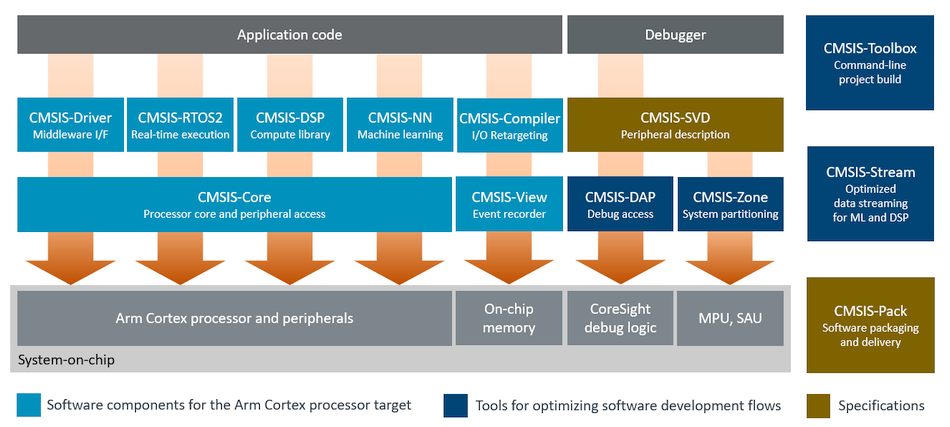
\includegraphics[scale=0.35]{presentation/cmsis_components.png}
\end{frame}

\begin{frame}{CMSIS-RTOS}
    \begin{itemize}
      \item C/C++ API for real-time operating systems
      \item Designed for Cortex M processors
      \item Version to use: CMSIS-RTOS2. It can be configured to use the CMSIS-RTX (or Keil RTX5), FreeRTOS, Zephyr, embOS, Azure Thread, and Micrium kernels.
      \item In SBM, version 2.1.3 is used, which is based on CMSIS v5 with RTX \href{https://arm-software.github.io/CMSIS_5/RTOS2/html/index.html}{(Documentation 2.1.3)}
      \item ARM has already released version 2.3.0, which is based on CMSIS V6 \href{https://arm-software.github.io/CMSIS_6/latest/RTOS2/index.html}{(Documentation 2.3.0)}
    \end{itemize}

\end{frame}
\section{CMSIS-RTOS: Features}
\begin{frame}{CMSIS-RTOS: Features}
    \begin{itemize}
  \item \textbf{Multithreaded applications}: based on the use of concurrent threads.
  \item Provides communication and synchronization mechanisms between threads.
  \item \textbf{Thread}:
    \begin{itemize}
        \item Portion of code that performs a specific function.
        \item Typically a function with an infinite loop and no return.
        \item The RTOS allows sharing execution with other threads.
        \item 5 states: \texttt{Running}, \texttt{Ready}, \texttt{Waiting/Blocked}, \texttt{Inactive}, \texttt{Terminated}.
    \end{itemize}
  \item \textbf{Scheduler}:
    \begin{itemize}
        \item Scheduling and sharing of CPU resources.
        \item Manages thread execution by allocating processor time (\texttt{SysTick}) to each thread.
    \end{itemize}
  \item \textbf{Timeslice}:
    \begin{itemize}
        \item Time period allocated to each thread.
        \item Multiple of the Tick (5 by default) generated by \texttt{SysTick} (1ms by default).
    \end{itemize}
\end{itemize}

\end{frame}

\begin{frame}{CMSIS-RTOS: Scheduler}
    \begin{itemize}
      \item \textbf{Preemptive}
          \begin{itemize}
            \item Preemption of "less priority" threads by "higher priority" threads.
          \end{itemize}
      \item \textbf{Round-Robin}
          \begin{itemize}
            \item All threads have the same priority.
            \item They run one after another in sequence during a "timeslice".
      \end{itemize}
      \item \textbf{Round-Robin Preemptive}
          \begin{itemize}
            \item Threads can have different priorities.
            \item Threads with equal priority run in Round-Robin fashion while there is no other higher priority thread in \texttt{READY} state.
            \item Be careful with priorities to avoid "hanging" the application.
            \item Default in CMSIS-RTOS - RTX.
      \end{itemize}
      \item \textbf{Cooperative Multitasking}
          \begin{itemize}
            \item All threads have equal priority.
            \item No Round-Robin.
            \item Each thread runs until it blocks (goes to \texttt{WAIT}) or until it yields execution to another thread (\texttt{yield}).
          \end{itemize}
    \end{itemize}
\end{frame}

\begin{frame}[fragile]{CMSIS-RTOS: Thread States}
    \begin{itemize}
        \item The OS scheduler is responsible for managing thread execution
        \item Thread states:
       \begin{itemize}
          \item \textbf{RUNNING}: thread currently executing.
          \item \textbf{READY}: threads ready to be executed. Once the running task has consumed its \textit{timeslice}, the next highest priority task becomes \textbf{RUNNING}.
          \item \textbf{BLOCKED/WAITING}: threads waiting for some event to occur.
          \item \textbf{TERMINATED}: threads that have finished but haven't released resources.
          \item \textbf{INACTIVE}: threads not created or terminated. They don't consume any resources.
        \end{itemize}
    \end{itemize}

\end{frame}
\begin{frame}{State Machine for a Thread}
    \begin{center}
        \resizebox{0.75\textwidth}{!}{
        \begin{tikzpicture}[shorten >=1pt, node distance=9cm, on grid, auto, font=\fontsize{18}{22}\selectfont, line width = 3pt]
          \node[state,  minimum size=3cm, fill=orange] (ready) {ready};
          \node[state,  minimum size=3cm, fill=green] (running) [right=of ready] {running};
          \node[state,  minimum size=3cm, fill=red] (blocked) [right=of running] {blocked};
          \node[state, minimum size=3cm, fill=gray!30] (inactive-terminated) [below=of running] {inactive-terminated};

          \path[->]
            (ready) edge  node {\textcolor{blue}{preempt}} (running)
            (ready) edge  node {terminate} (inactive-terminated)
            (inactive-terminated) edge  node {create} (ready)
            (running) edge  node {preempt} (ready)
            (blocked) edge [bend left] node {events occur} (running)
            (running) edge [bend left] node {\textcolor{blue}{wait}} (blocked)
            (blocked) edge [bend right] node {events occur} (ready)
            (blocked) edge [bend left] node {terminate} (inactive-terminated)
            (running) edge node {terminate} (inactive-terminated)
            (inactive-terminated) edge node {create} (running);
        \end{tikzpicture}
        }
    \end{center}
\end{frame}
\section{Basic Code}
\begin{frame}[fragile]{Thread in Keil Microvision}
    \begin{minted}[fontsize=\scriptsize, bgcolor=blue!5]{c}
    #include "cmsis_os2.h"

    osThreadId_t tid_thread; // tid_thread identifies the thread. It will be used in specific RTOS functions
    ...

    tid_Thread = osThreadNew(Thread, NULL, NULL);
    if (tid_Thread == NULL) {
        return(-1);
    }

void Thread (void *argument){
        // insert code that you only want to execute once
        while(1){
        // insert code that you want to execute continuously

        }
        // this point is never reached in this example

    }
    \end{minted}
    \begin{itemize}
        \item It is highly advisable to create a header file where the startup function should be declared so it can be used by other software modules

    \end{itemize}
\end{frame}

\begin{frame}[fragile]{Application Implementation with Threads}
    \begin{columns}
        \begin{column}{0.50\textwidth}
            \begin{minted}[fontsize=\scriptsize, bgcolor=blue!5]{c}
// File with thread ThDisplay.c
#include "cmsis_os2.h"
#include "ThDisplay.h"

osThreadId_t tid_ThDisplay;
...

tid_ThDisplay = osThreadNew(ThDisplay,
                NULL, NULL);
if (tid_ThDisplay == NULL) {
    return(-1);
}

void ThDisplay (void *argument){
    int ciclo=0;
    Init_display();
    while(1){
    .....

    }

}
            \end{minted}
        \end{column}
    \begin{column}{0.50\textwidth}
        \begin{minted}[fontsize=\scriptsize, bgcolor=blue!5]{c}
        // File main.c
        #include "ThDisplay.h"
        int main(void){
            int status=0;
            HAL_Init();
            SystemClock_Config();
            SystemCoreClockUpdate();
        #ifdef RTE_CMSIS_RTOS2
            oskernelInitilize();
            status|= Init_ThDisplay();
            osKernelStart();
        #endif
        }
        \end{minted}
        \begin{minted}[fontsize=\scriptsize, bgcolor=blue!5]{c}
        // Header file ThDisplay.h
        #include "stm32f4xx_hal.h"

        #ifndef __THDISPLAY__H
        #define __THDISPLAY__H
            #define S_PINTA  0x0001U
            int Init_ThDisplay(void);
        #endif

        \end{minted}
    \end{column}
    \end{columns}
    \begin{itemize}
        \item It is highly advisable to create a header file where the initialization function should be declared so it can be used by other software modules

    \end{itemize}
\end{frame}
\section{Synchronization}
\begin{frame}{CMSIS RTOS Synchronization}
    \begin{columns}
        \begin{column}{0.50\textwidth}
            \begin{itemize}
                \item An application will use multiple threads and resources that need to be synchronized
                \item What is the problem?
                    \begin{itemize}
                        \item Multiple threads run concurrently and want to use the same shared resource, which can be software or hardware
                        \item Sequential use of the shared resource must be guaranteed
                    \end{itemize}
                \item What is the solution?
                \begin{itemize}
                    \item Use resources such as events, flags, queues, semaphores, etc.
                    \item CMSIS-RTOS V2 implements an API with these resources
                \end{itemize}
            \end{itemize}
        \end{column}
        \begin{column}{0.50\textwidth}
            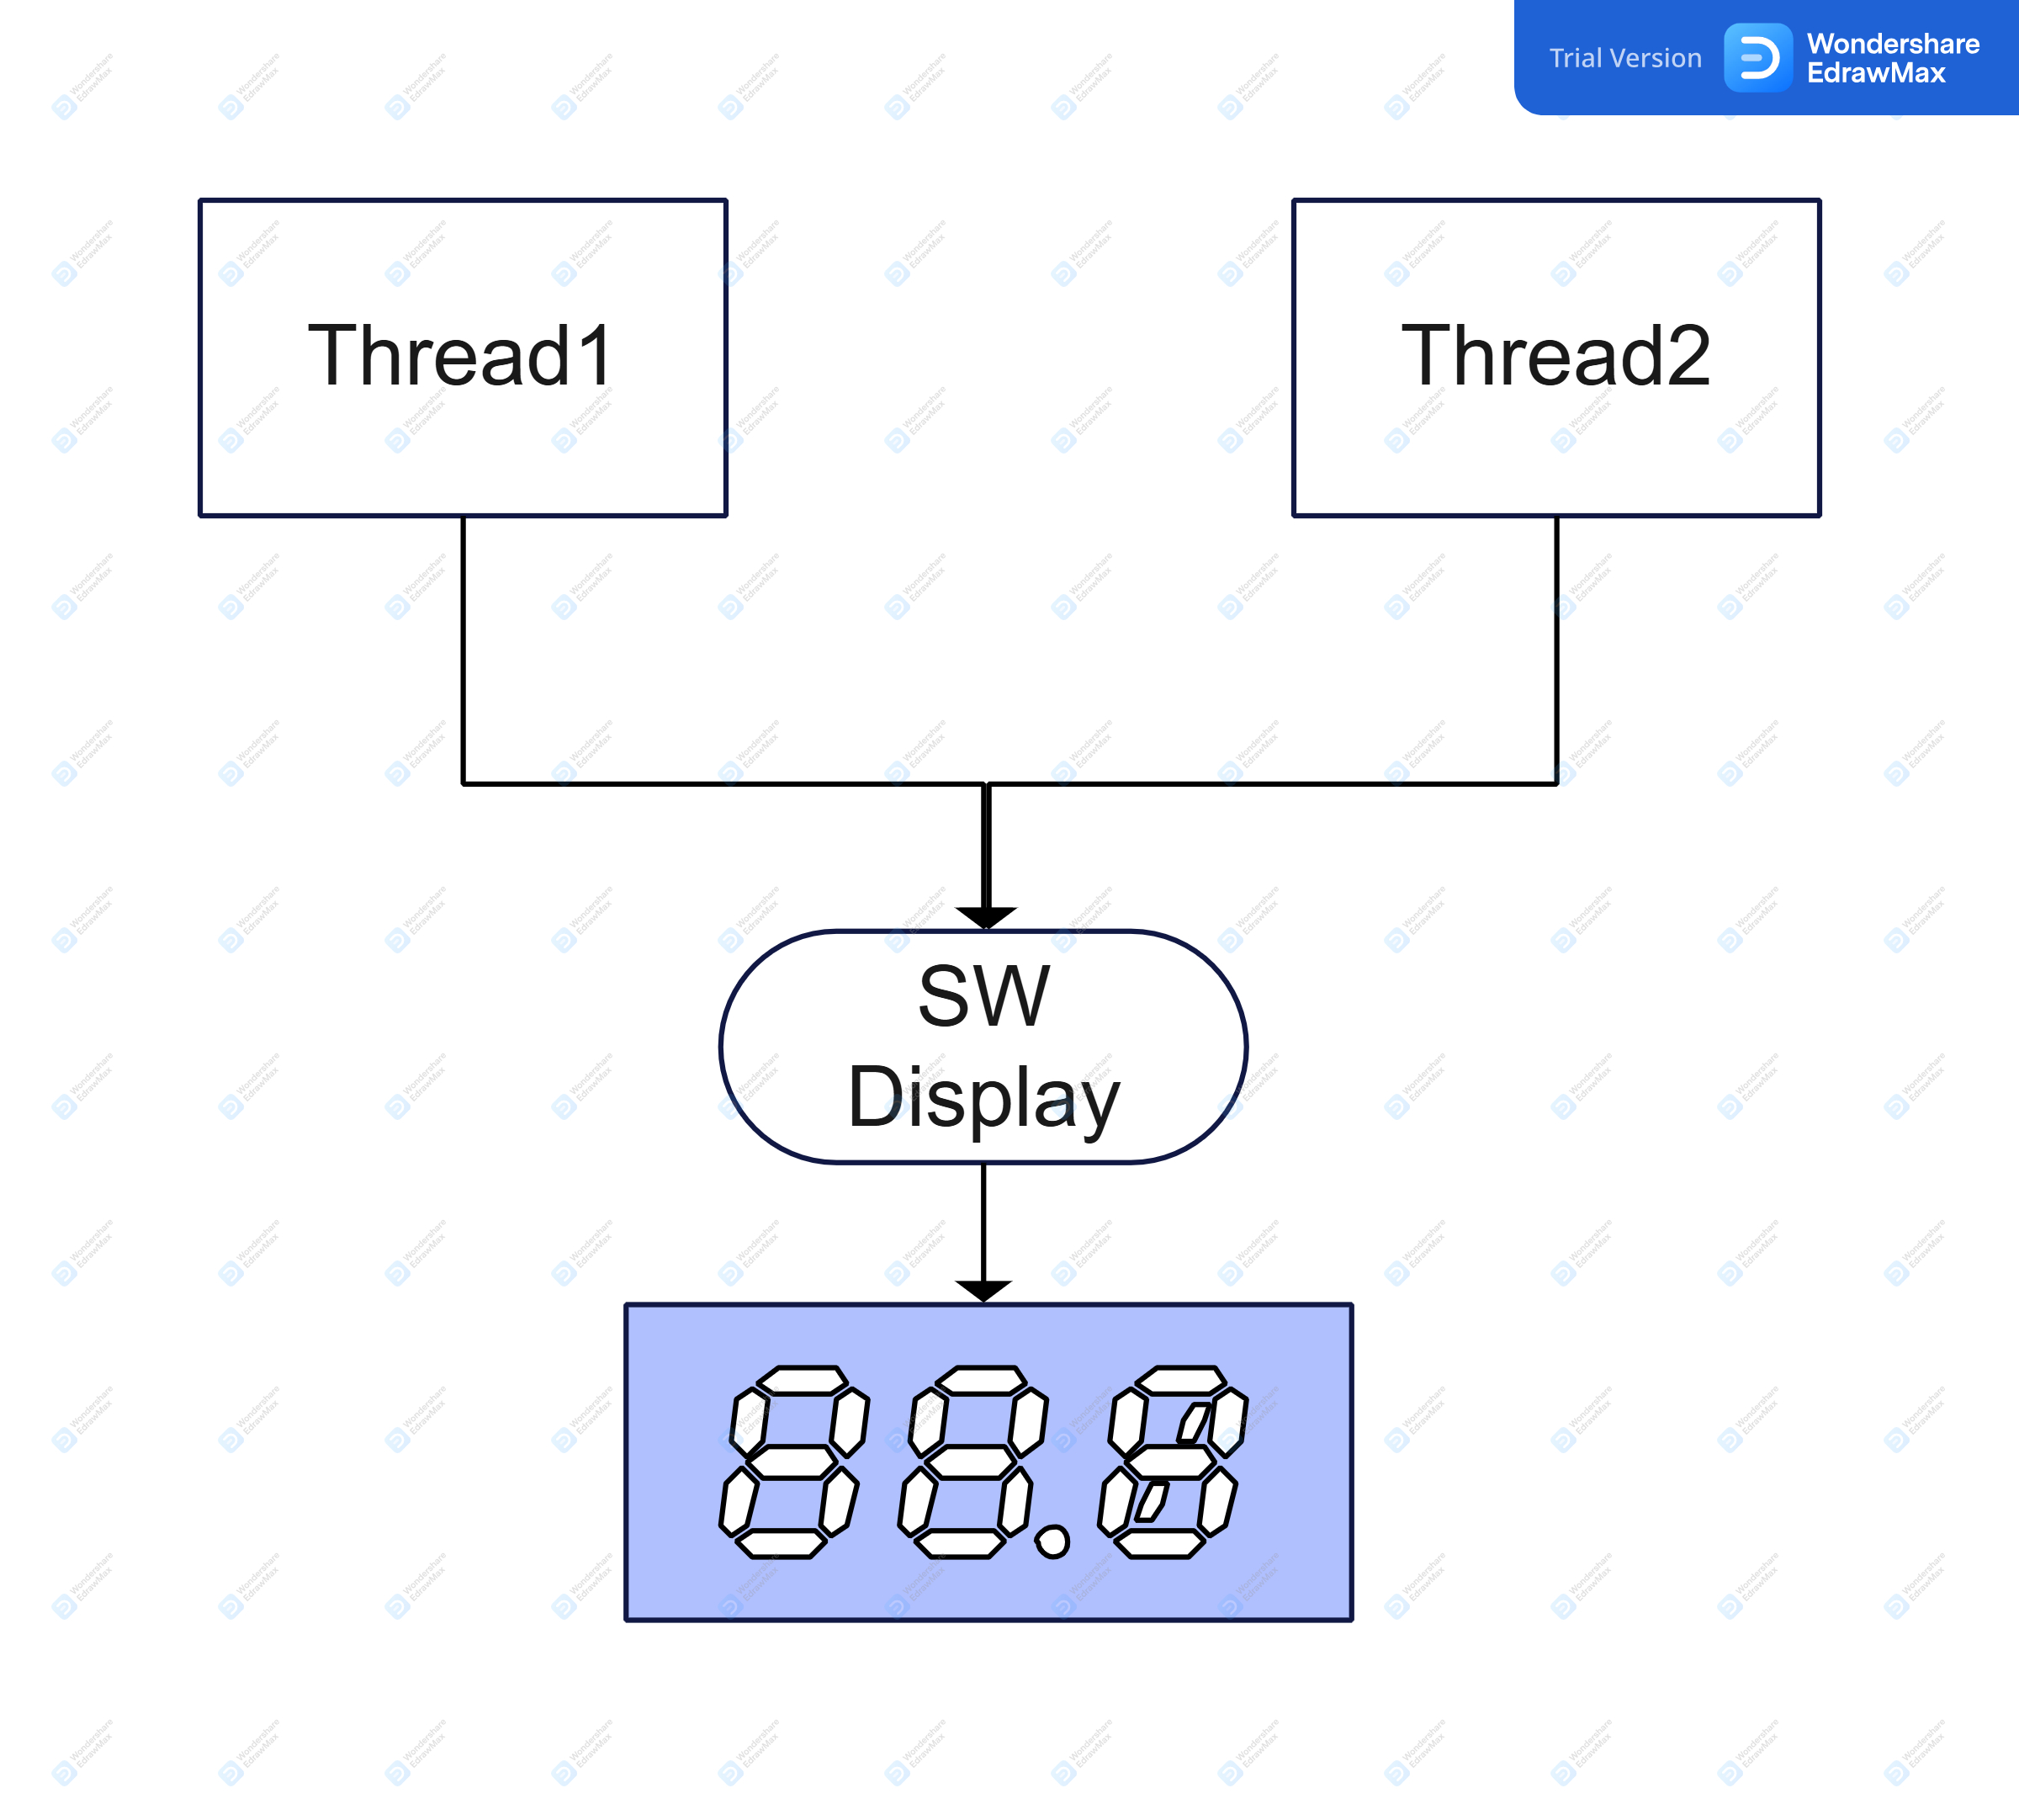
\includegraphics[scale=0.05]{presentation/threads.jpg}
        \end{column}
    \end{columns}
\end{frame}
\begin{frame}{CMSIS RTOS Synchronization}
    \begin{columns}
        \begin{column}{0.50\textwidth}
            \begin{itemize}
                \item A possible solution: A queue managed by the Operating System is added
                \item There is a thread that reads messages arriving at the queue to send them to the display
                \item Each thread that wants to send a message to the LCD writes to the queue
            \end{itemize}
        \end{column}
        \begin{column}{0.50\textwidth}
            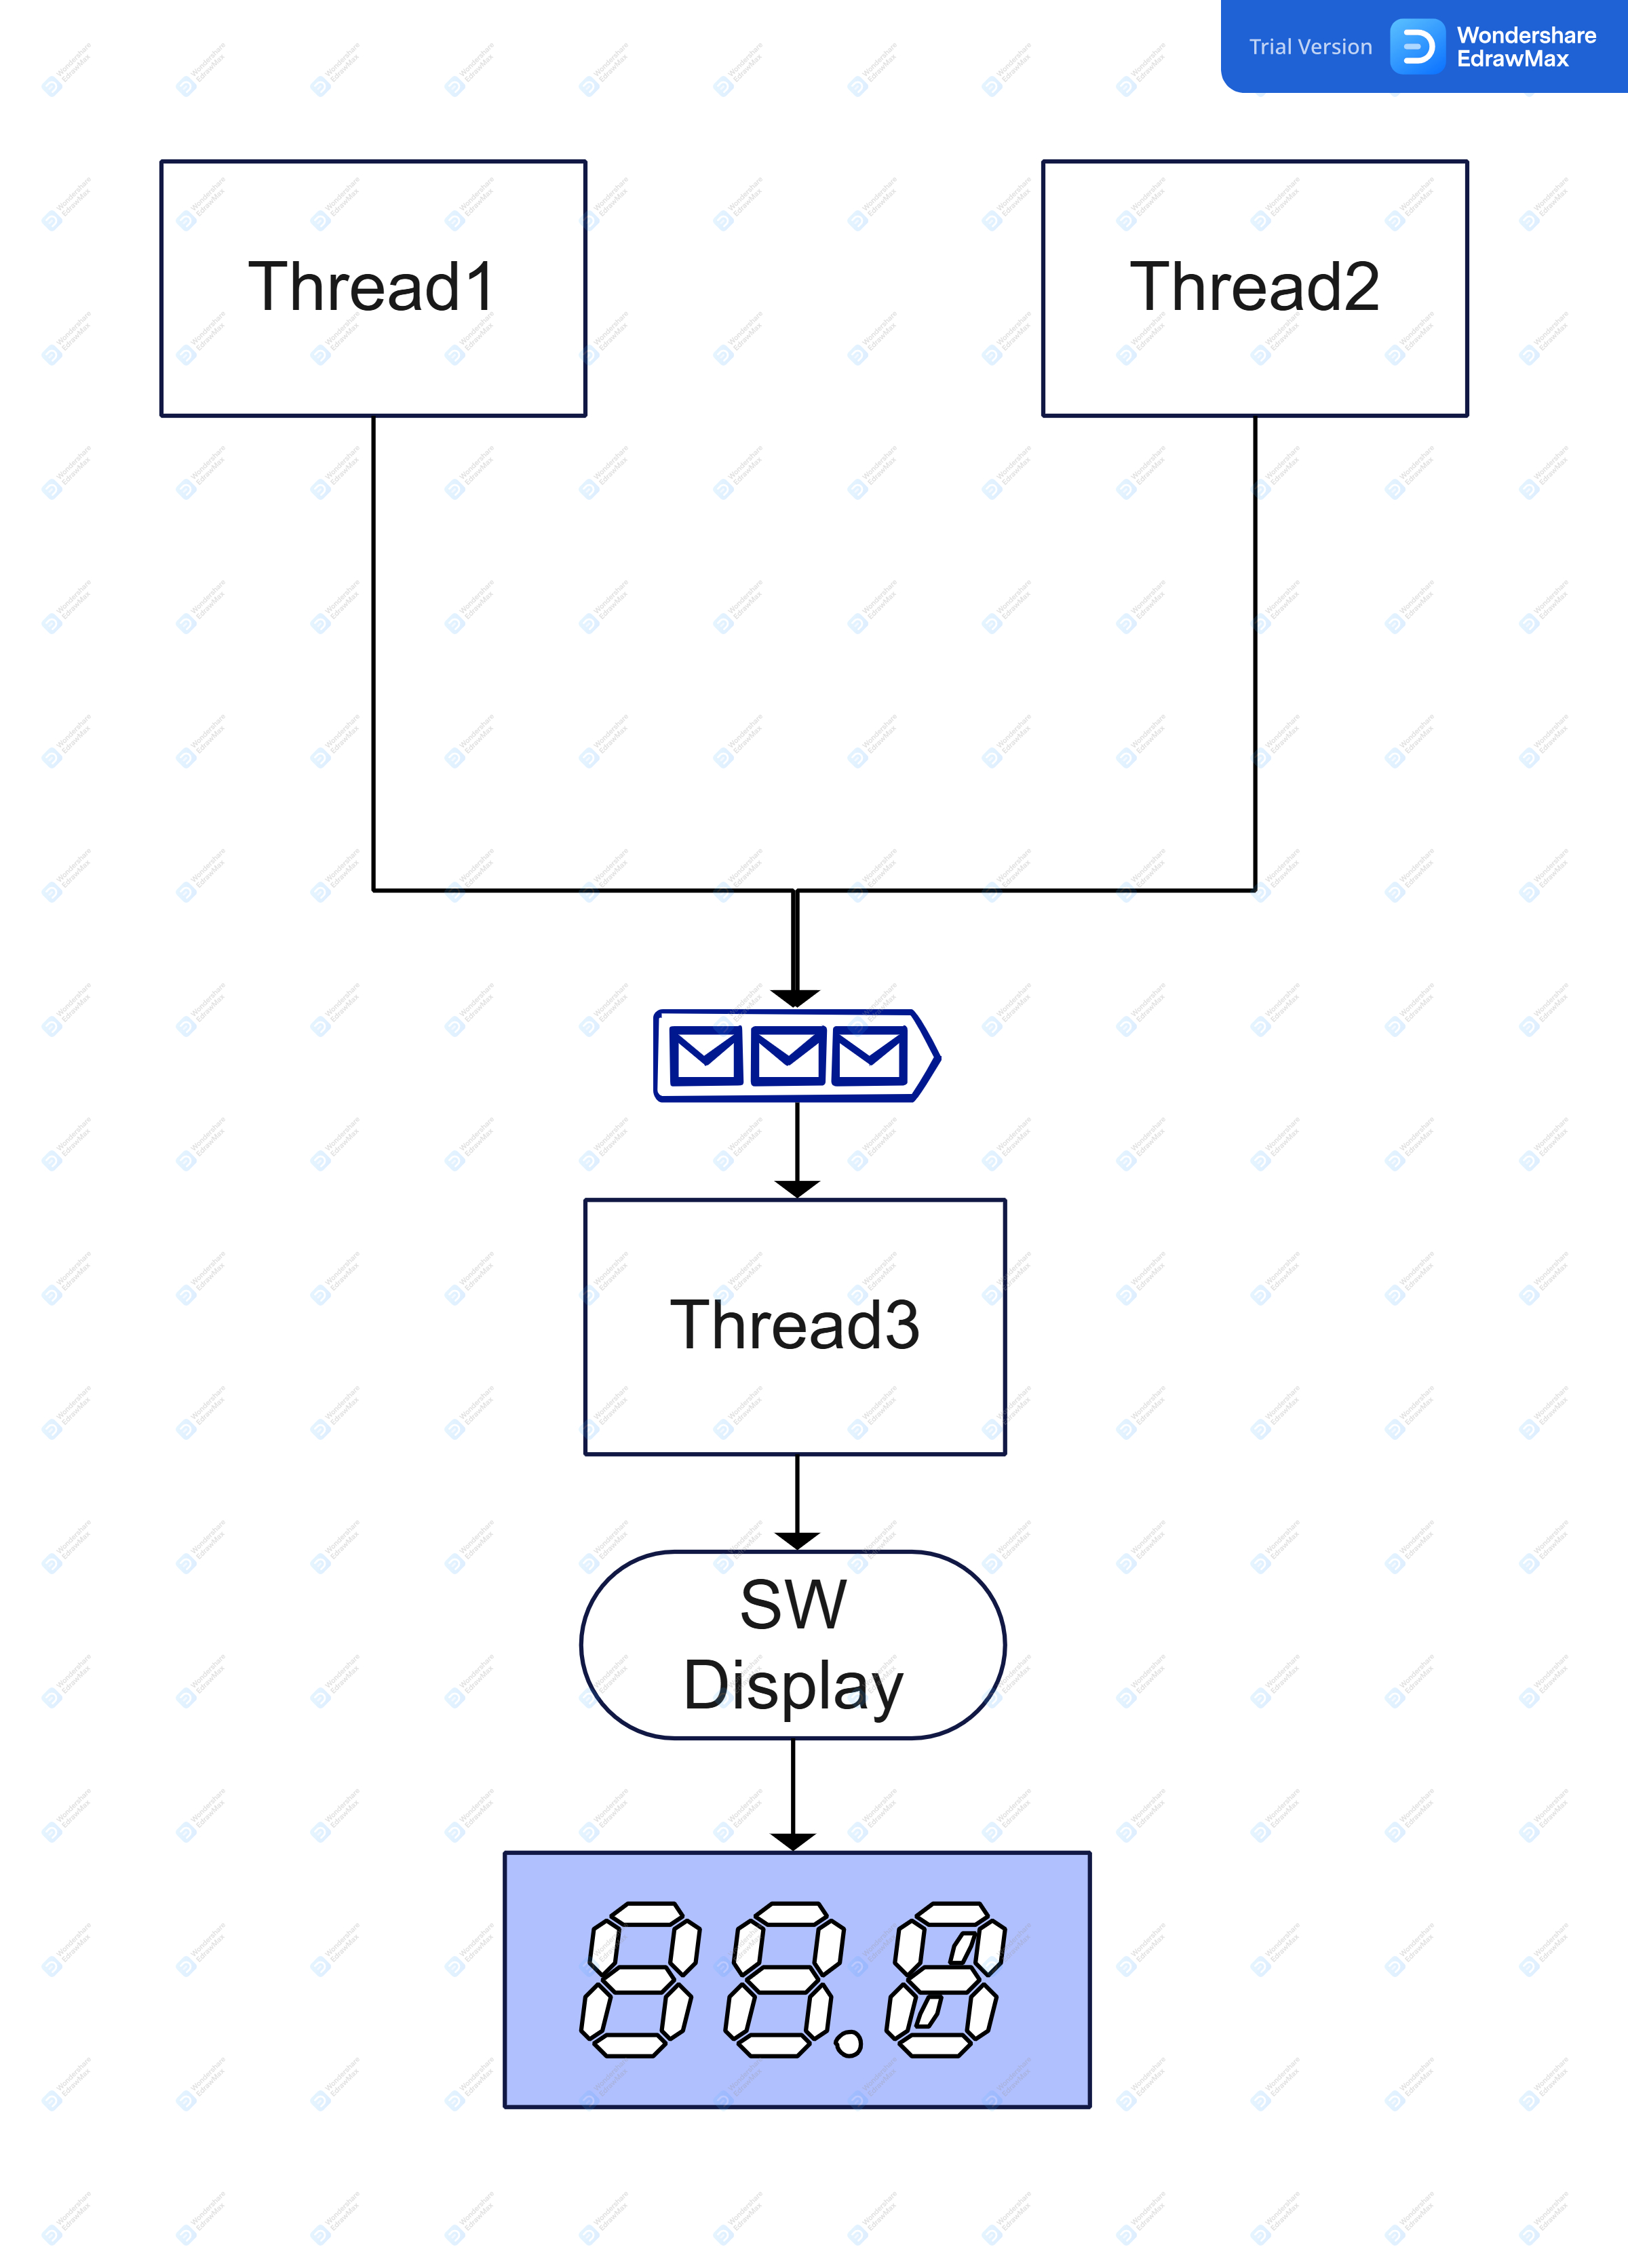
\includegraphics[scale=0.05]{presentation/threads-sync.jpg}
        \end{column}
    \end{columns}
\end{frame}

\begin{frame}[fragile]{Synchronization with Thread Flags}
      \begin{itemize}
          \item \textbf{Problem:} Task 1 periodically generates events/data (1s). We want task 2 to only execute when data is available and not consume CPU while waiting.
      \end{itemize}
      \begin{columns}
            \begin{column}{0.50\textwidth}
                \begin{itemize}
                    \item[]
                    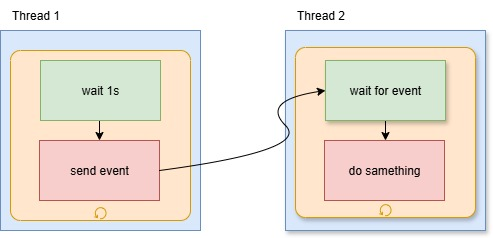
\includegraphics[scale=0.25]{presentation/flags.jpg}
                    \item Thread 2 enters the \textbf{Waiting} state until Thread 1 activates the flag.
                    \item When the flag or flag set is activated, the thread enters the \textbf{Ready} state
                \end{itemize}
            \end{column}
            \begin{column}{0.50\textwidth}
             \begin{minted}[fontsize=\scriptsize, bgcolor=blue!5]{c}
void Thread1 (void *argument){
    while(1){
    osdelay(1000);
    osThreadFlagSet(tid_thread2, 0x0001);
    }
}

void Thread2 (void *argument){
    while(1){
    status = osThreadFlagWait(0x0001,
             osFlagsWaitAny,
             osWaitForever);
    //
    }
}
             \end{minted}

            \end{column}
     \end{columns}
\end{frame}

\begin{frame}[fragile]{CMSIS RTOS Thread Flags}

    \begin{itemize}
        \item []
         \begin{minted}[fontsize=\scriptsize, bgcolor=blue!5]{c}
uint32_t osThreadFlagSet(osThreadId_t thread_id, uint32_t flags)
/* Sets the specified flag of an active thread
Can be called from an interrupt */

         \end{minted}
         \begin{minted}[fontsize=\scriptsize, bgcolor=blue!5]{c}
uint32_t osThreadFlagClear(osThreadId_t thread_id, uint32_t signals)
/* Clears the specified flag of an active thread
Cannot be called from an interrupt */

         \end{minted}
         \begin{minted}[fontsize=\scriptsize, bgcolor=blue!5]{c}
uint32_t osThreadFlagsWait(uint32_t flags, uint32_t options, uint32_t timeout)
/* Waits for one or more flags to continue execution
Cannot be called from an interrupt */

         \end{minted}
         \begin{minted}[fontsize=\scriptsize, bgcolor=blue!5]{c}
uint32_t osThreadFlagGet(void)
/* Returns the flags of the running thread
Cannot be called from an interrupt */

         \end{minted}
         \item[] \href{https://arm-software.github.io/CMSIS_5/RTOS2/html/group__CMSIS__RTOS__ThreadFlagsMgmt.html}{CMSIS RTOS V2 Thread Flags reference}
    \end{itemize}
\end{frame}

\begin{frame}[fragile]{CMSIS RTOS Queues}
\begin{itemize}
    \item Producer/Consumer concept. A Thread or an ISR produces data and a thread consumes it
\end{itemize}
\begin{columns}
  \begin{column}{0.45\textwidth}
    \begin{minted}[fontsize=\tiny, bgcolor=blue!5]{c}
int Init_Thread (void) {
  id_MsgQueue = osMessageQueueNew(16,
                sizeof(uint8_t), NULL);
  tid_Thread = osThreadNew(Producer, NULL, NULL);
  if (tid_Thread == NULL) {   return(-1);  }
  tid_Thread = osThreadNew(Consumer, NULL, NULL);
  if (tid_Thread == NULL) {   return(-1);  }
  return(0);
}
void Producer (void *argument) {
    uint8_t index=0;
    osStatus_t status;
        while (1) {
        status=osMessageQueuePut(id_MsgQueue,
                             &index, 0U, 0U);
        	index++;
        	osDelay(100);
        }
}
void Consumer (void *argument) {
while (1) {
	status = osMessageQueueGet(id_MsgQueue,
               &val, NULL, osWatiForever );
  }
}

    \end{minted}
    \end{column}
    \begin{column}{0.55\textwidth}
     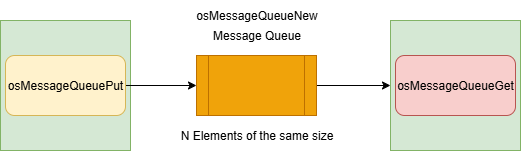
\includegraphics[scale=0.35]{presentation/queues.drawio.png}
    \end{column}
\end{columns}
\end{frame}

\begin{frame}[fragile]{CMSIS RTOS Queues}
    \begin{itemize}
        \item []
         \begin{minted}[fontsize=\scriptsize, bgcolor=blue!5]{c}
osMessageQueueId_t 	osMessageQueueNew (uint32_t msg_count, uint32_t msg_size, const osMessageQueueAttr_t *attr)
/* Create and Initialize a Message Queue object */
         \end{minted}
         \begin{minted}[fontsize=\scriptsize, bgcolor=blue!5]{c}
const char * 	osMessageQueueGetName (osMessageQueueId_t mq_id)
/* Get name of a Message Queue object. */
         \end{minted}
         \begin{minted}[fontsize=\scriptsize, bgcolor=blue!5]{c}
osStatus_t 	osMessageQueuePut (osMessageQueueId_t mq_id, const void *msg_ptr, uint8_t msg_prio, uint32_t timeout)
/* Put a Message into a Queue or timeout if Queue is full */
         \end{minted}
         \begin{minted}[fontsize=\scriptsize, bgcolor=blue!5]{c}
osStatus_t 	osMessageQueueGet (osMessageQueueId_t mq_id, void *msg_ptr, uint8_t *msg_prio, uint32_t timeout)
/* Get a Message from a Queue or timeout if Queue is empty */
         \end{minted}
         \begin{minted}[fontsize=\scriptsize, bgcolor=blue!5]{c}
uint32_t 	osMessageQueueGetCapacity (osMessageQueueId_t mq_id)
/* Get maximum number of messages in a Message Queue */
         \end{minted}
         \begin{minted}[fontsize=\scriptsize, bgcolor=blue!5]{c}
uint32_t 	osMessageQueueGetMsgSize (osMessageQueueId_t mq_id)
/* Get maximum message size in a Message Queue */
         \end{minted}
         \begin{minted}[fontsize=\scriptsize, bgcolor=blue!5]{c}
uint32_t 	osMessageQueueGetCount (osMessageQueueId_t mq_id)
/* 	Get number of queued messages in a Message Queue */
         \end{minted}
         \begin{minted}[fontsize=\scriptsize, bgcolor=blue!5]{c}
uint32_t 	osMessageQueueGetSpace (osMessageQueueId_t mq_id)
/* Get number of available slots for messages in a Message Queue */
         \end{minted}
         \begin{minted}[fontsize=\scriptsize, bgcolor=blue!5]{c}
osStatus_t 	osMessageQueueReset (osMessageQueueId_t mq_id)
/* Reset a Message Queue to initial empty state */
         \end{minted}
         \begin{minted}[fontsize=\scriptsize, bgcolor=blue!5]{c}
osStatus_t 	osMessageQueueDelete (osMessageQueueId_t mq_id)
/* 	Delete a Message Queue object */
         \end{minted}

         \item[] \href{https://arm-software.github.io/CMSIS_5/RTOS2/html/group__CMSIS__RTOS__Message.html}{CMSIS RTOS V2 Thread Message Queue reference}
    \end{itemize}
\end{frame}

\begin{frame}[fragile]{CMSIS Delays and Timed Actions by \textbf{Software}}
\begin{itemize}
    \item Generic wait functions based on SysTick Timer
    \begin{minted}[fontsize=\scriptsize, bgcolor=blue!5]{c}
osStatus_t status;
uint32_t delayTime=1000;
status = osdelay(delayTime); // task that blocks until time elapses
uint32_t tick;

tick = oskernelGetTickCount(); // gets current system tick value
for (;;){
    tick += 1000u;
    osdelayUnyil(tick); // Waits until 1000 ticks pass
}
    \end{minted}
    \item \textbf{These functions cannot be used from interrupt service routines}
    \item Virtual timers
        \begin{itemize}
            \item Execute a function (\textbf{callback}) when time expires
            \item The callback function is user-defined
        \end{itemize}
\end{itemize}

\end{frame}

\begin{frame}[fragile]{CMSIS-RTOS Virtual Timers}
    \begin{columns}
        \begin{column}{0.55\textwidth}
        \begin{itemize}
        \item Virtual timers have two operating modes:
        \begin{itemize}
            \item \textbf{one-shot} The timer is started and after a configurable time (in Ticks steps) a callback is executed,
            \item \textbf{periodic} The timer is started and each time the configured time elapses, the callback is executed
            \item These virtual timers cannot (and should not) be configured to run with times below ms
        \end{itemize}
        \end{itemize}
        \end{column}
        \begin{column} {0.45\textwidth}
        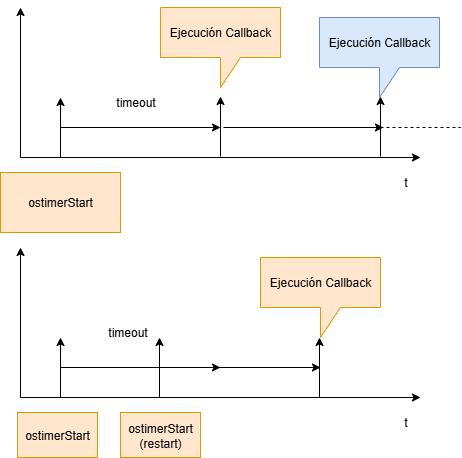
\includegraphics[scale=0.25]{presentation/softwaretimers.drawio.png}
     \end{column}
    \end{columns}
\end{frame}

\begin{frame}[fragile]{CMSIS-RTOS Virtual Timers}
    \begin{columns}
        \begin{column}{0.65\textwidth}
            \begin{minted}[fontsize=\scriptsize, bgcolor=blue!5]{c}
osTimerId_t swtim_id;
static uint32_t param=0;
/* Timer callback function */
void TimerLed_Callback (void const *arg){
    LED_Toggle(LED1);
}

/* Timer initialization and start */
int Init_SWTImer (void){
    osStatus_t status;
    Init_LED(LED1);
    param=3;
    swtim_id = osTimerNew((osTimerFunc_t)&TimerLed_Callback,
                          osTimerPeriodic, &param, NULL);
    if (swtim_id != NULL){
        status = osTimerStart(swtim_id, 1000U);
        if (status != osOk){
            return -1;
        }
    }
return 0;
}

        \end{minted}
     \end{column}
     \begin{column}{0.35\textwidth}
         \begin{itemize}
             \item The timer identifier is used by the function that starts it
             \item The timer can be configured as osTimerPeriodic or osTimerOnce
         \end{itemize}
     \end{column}
    \end{columns}
\end{frame}

\begin{frame}[fragile]{CMSIS RTOS Timers Software}
    \begin{itemize}
        \item These functions \textbf{cannot be called from interrupt routines}
        \item[]
        \item[]
         \begin{minted}[fontsize=\scriptsize, bgcolor=blue!5]{c}
osTimerId_t 	osTimerNew (osTimerFunc_t func, osTimerType_t type, void *argument, const osTimerAttr_t *attr)
/* Create and Initialize a timer. */
         \end{minted}
         \begin{minted}[fontsize=\scriptsize, bgcolor=blue!5]{c}
const char * 	osTimerGetName (osTimerId_t timer_id)
/* Get name of a timer. */
         \end{minted}
         \begin{minted}[fontsize=\scriptsize, bgcolor=blue!5]{c}
osStatus_t 	osTimerStart (osTimerId_t timer_id, uint32_t ticks)
/* Start or restart a timer. */
         \end{minted}
         \begin{minted}[fontsize=\scriptsize, bgcolor=blue!5]{c}
osStatus_t 	osTimerStop (osTimerId_t timer_id)
/* Stop a timer */
         \end{minted}
         \begin{minted}[fontsize=\scriptsize, bgcolor=blue!5]{c}
uint32_t 	osTimerIsRunning (osTimerId_t timer_id)
/* Check if a timer is running. */
         \end{minted}
         \begin{minted}[fontsize=\scriptsize, bgcolor=blue!5]{c}
osStatus_t 	osTimerDelete (osTimerId_t timer_id)
/* Delete a timer. */
         \end{minted}

         \item[] \href{https://arm-software.github.io/CMSIS_5/RTOS2/html/group__CMSIS__RTOS__TimerMgmt.html}{CMSIS RTOS V2 Thread Message Queue reference}
    \end{itemize}
\end{frame}
\section{Configuration and Other Tools}
\begin{frame}{Structure of Projects Using CMSIS-RTOS}
\resizebox{0.9\textwidth}{!}{
\begin{forest}
for tree={
    grow'=south,
    draw,
    rectangle,
    node options={align=center, font=\Huge\ttfamily, inner sep=14pt},
    edge path={
        \noexpand\path [draw, \forestoption{edge}] (!u.parent anchor) --  (.child anchor)\forestoption{edge label};
    },
}
[Project
  [Source Group 1
    [main.c]
    [utils.c]
    [More files]
  ]
  [\textcolor{red}{CMSIS}
    [rtx\_lib.c]
    [RTX\_Config.c]
    [\textcolor{green}{RTX\_Config.h}]
    [More files]
  ]
  [Device
    [stm32f4xx\_hal.c]
    [More files]
  ]
]
\end{forest}}
\begin{itemize}
    \item The figure only shows some files
    \item The \textcolor{green}{RTX\_Config.h} file allows configuring the OS parameters
\end{itemize}
\end{frame}

\begin{frame}{CMSIS-RTOS Configuración de parámetros}

\begin{table}[H]
\centering
\begin{tabular}{|l|l|}
\hline
\multicolumn{2}{|c|}{\textbf{Configuración del Sistema}} \\
\hline
Global Dynamic Memory Size & Tamaño de la memoria\\
kernel Tick Frequency & Frecuencia del tick sistema (Hz) \\
Round-Robin Thread Switching & Activar Round-Robin \\
Round-Robin Timeout & Tiempo de cambio de hilo \\
ISR FIFO QUEUE & Tamaño de cola FIFO para ISR \\
\hline
\multicolumn{2}{|c|}{\textbf{Configuración de Hilos}} \\
\hline
Default Thread Stack Size & Tamaño por defecto de pila de hilo \\
IDLE THREAD STACK SIZE & Pila del hilo idle \\
\hline
\multicolumn{2}{|c|}{\textbf{Timers}} \\
\hline
Timer Thread Priority & Prioridad del thread para los timers virtuales \\
Tamaño del stack & Pila del hilo de temporizador \\
OS\_TIMER\_THREAD\_TCB\_SIZE & TCB del hilo de temporizador \\
\hline
\end{tabular}
\caption{Some of the configurable parameters in RTX\_Config.h grouped by category}
\end{table}

\end{frame}

\begin{frame}{Watch Window RTX}
    \begin{itemize}
        \item Allows visualization of RTX operating system objects created with CMSIS-RTOS
        \begin{columns}
            \begin{column}{0.50\textwidth}
            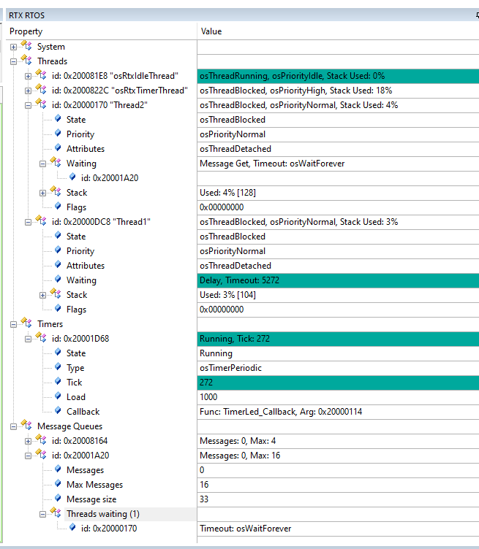
\includegraphics[scale=0.5]{presentation/watchwindowRTX.png}

            \end{column}
            \begin{column}{0.50\textwidth}
            \begin{itemize}
                \item osRtxidleThread OS idle task
                \item osRtxTimerThread Thread that manages virtual timers
                \item Thread1, Thread2, Threads created in the application
                \item Timers. id: 0x20001D68 Example of a periodic timer with its details
                \item Message Queues. id: 0x20008164. Example queue with size 4. id: 0x20001A20. Queue with 16 message capacity. Each message occupies 33 bytes. The thread with id:0x20000170 is blocked waiting for a message in this queue

            \end{itemize}
            \end{column}
        \end{columns}
    \end{itemize}
\end{frame}
\section{Final Considerations}
\begin{frame}{CMSIS-RTOS Considerations}
\begin{itemize}
    \item Before addressing an application, its structure will be designed so that, as much as possible, each peripheral will be managed by a software module composed of the corresponding thread, signals, queues, and data structures.
    \item ISRs will be handled by the HAL, and in the respective Callbacks (pay attention to the Callbacks that can be defined with CMSIS-Driver for I2C/SPI and UART), the necessary signals and messages will be sent to the different threads. They will be short routines and loops will be avoided. Monitor which OS elements can be implemented within them.
    \item Pay special attention to synchronization between threads.
    \item The use of global variables will be minimized as much as possible.
\end{itemize}

\end{frame}
\begin{frame}{Exercises to Understand the Use of CMSIS RTOS V2}
    \begin{itemize}
        \item Available on github \href{https://github.com/mruizlgz/SBM-rtos}{(sbm-rtos)}. Documentation at: \href{https://mruizglz.github.io/SBM-rtos}{(SPHINX DOC)} or \href{https://mruizglz.github.io/SBM-rtos/simplepdf/SBM-CMSIS-RTOS-V2.pdf}{(PDF)}

        \item Examples:
            \begin{itemize}
                \item threads Creation of two threads using the same function
                \item threads-flags Synchronization with flags
                \item threads-queues Synchronization with queues
                \item threads-timers Use of virtual timers
            \end{itemize}
    \end{itemize}
\end{frame}
